\section{The Metaphysics of Deliquescence}

\begin{wrapfigure}{rt}{.3\textwidth}
 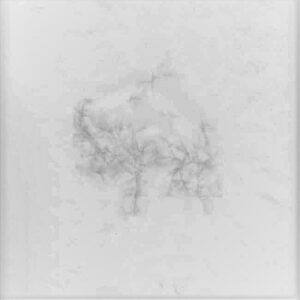
\includegraphics[scale=.5]{a20060629TheMetaphysicsofDeliquescence-img001.jpg} 
\caption{Deliquescence}
\end{wrapfigure} 

\textbf{del·i·ques·cence} \emph{n} The process of dissolving or of becoming liquid through the absorption of moisture from the atmosphere.

\paragraph{Form and Formlessness}
The new and interesting artist — \textbf{Jillian Taylor}\footnote{\url{https://www.facebook.com/search/top?q=jilli-art}}, in her series on \emph{deliquescence} writes:

\begin{quotex}
A container is often presented as an appealing package concealing something great inside, while it may simply be a small structure enclosing an allotted and restricted space. These simple boxlike structures of confinement are the product of a given set of instructions, compiled of rigid diagrammatic lines and shapes. As each instruction is followed, a permanent fold is pressed simultaneously, and the result is an enclosed structure of folds. Echoes of one's thoughts repeatedly bounce inside their confines. In an abandonment of the given instructions, the containers are unfolded and discarded. Through the folds, a constant reminder of the followed directions, will never disappear. 

\end{quotex}
A myth in the Sorelian sense is not mere intellectual assent to a worldview. It is a power-idea and, as such, is an effective motivation to action. The myth is also presented as an appealing package, which then shapes its ``contents" — those who believe.

\begin{quotex}
Memories begin to unintentionally fade as a result of acceptance and the new state of refinement. As the represented memories fade, the existing creases and folds begin to flatten and dissolve into their surrounding spaces. Specific moments linger, creating the potential for faded moments to resurface before fully dissipating. 

\end{quotex}
So everything and everyone is placed into a container of a political correctness, then deliquesces into formlessness, taking on the shape of the container and losing any vestigial memory of prior differentiations.

Yet absolute formlessness, the equivalent of non-existence, is metaphysically impossible, so there is always ``the potential for faded moments to resurface".



\flrightit{Posted on 2006-06-29 by Cologero }
